\documentclass[tikz,border=25pt]{standalone}
\usepackage{amsmath, amssymb}
\usetikzlibrary{matrix, positioning, fit, backgrounds, calc}

\begin{document}
	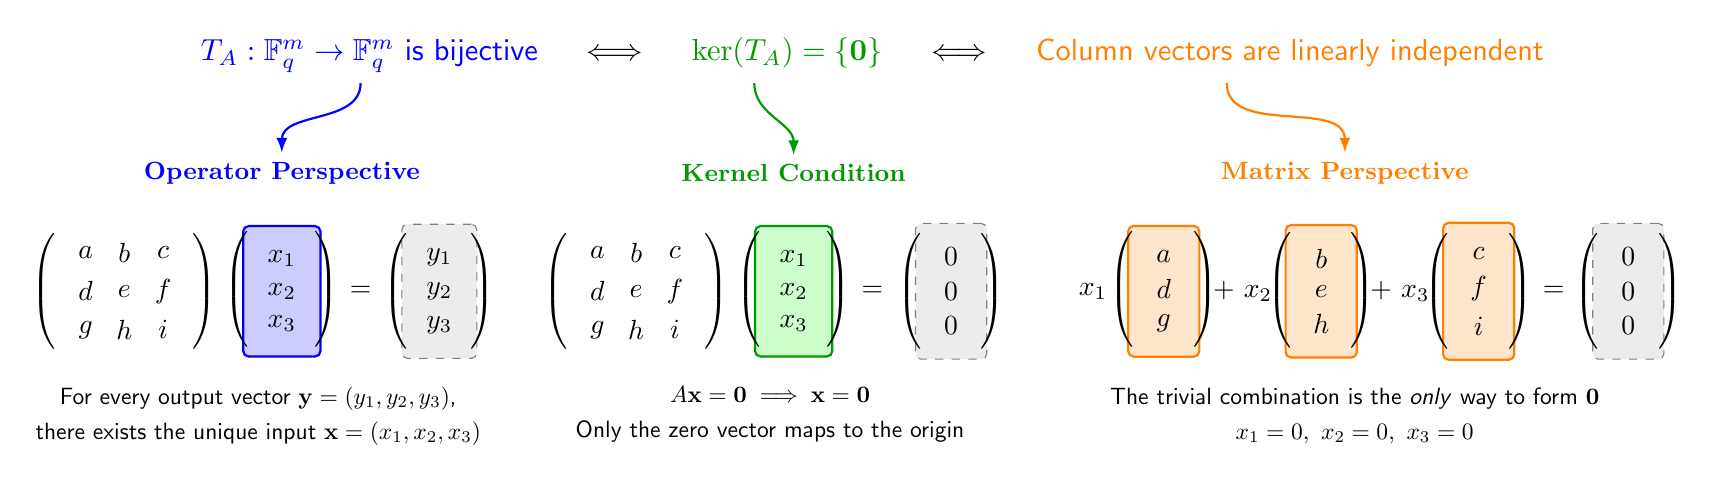
\begin{tikzpicture}[
		font=\sffamily,
		% Style for the matrices
		mtx/.style={
			matrix of math nodes,
			left delimiter=(, right delimiter=),
			nodes={minimum width=1.2em, inner sep=2pt, anchor=center},
			column sep=2pt, row sep=2pt,
			ampersand replacement=\&
		},
		% Highlighting styles for active columns
		hl-v1/.style={fill=blue!20, draw=blue, thick, rounded corners=2pt},
		hl-v2/.style={fill=orange!20, draw=orange, thick, rounded corners=2pt},
		hl-v3/.style={fill=green!20, draw=green!60!black, thick, rounded corners=2pt},
		hl-v4/.style={fill=purple!20, draw=purple, thick, rounded corners=2pt},
		% Style for the accumulating "Span Box"
		hl-span/.style={fill=gray!15, draw=gray, dashed, rounded corners=2pt},
		% Title & Text
		mainTitle/.style={font=\sffamily\bfseries\LARGE, color=darkgray, align=center},
		term label/.style={font=\bfseries\small, align=center}
		]
		
		% ==============================================================================
		% MAIN TITLE
		% ==============================================================================
%		\node[mainTitle] (title) at (0, 7.5) {Structural Equivalence:\\Bijectivity, Trivial Kernel, and Linear Independence};
		
		% --- 1. The Main Equation ---
		\node[scale=1.1] (eq) at (1.5, 3) {
			\textcolor{blue}{$T_A:\mathbb{F}_q^m\to \mathbb{F}_q^m \text{ is bijective}$} \quad $\iff$ \quad 
			\textcolor{green!60!black}{$\ker(T_A) = \{\mathbf{0}\}$} \quad $\iff$ \quad 
			\textcolor{orange}{Column vectors are linearly independent}
		};
		
		% ==============================================================================
		% ROW 1: THE THREE EQUIVALENT VIEWS
		% ==============================================================================
		
		% === Branch 1: Bijection (Blue) ===
		\begin{scope}[shift={(-6.5, 0)}, scale=1]
			\node[term label, text=blue] (lbl1) at (0.5, 1.5) {Operator Perspective};
			
			\matrix[mtx] (M_bij_A) at (-1.5, 0) {
				a \& b \& c \\
				d \& e \& f \\
				g \& h \& i \\
			};
			\matrix[mtx] (M_bij_x) at (0.5, 0) { x_1 \\ x_2 \\ x_3 \\ };
			\node at (1.5, 0) {$=$};
			\matrix[mtx] (M_bij_y) at (2.5, 0) { y_1 \\ y_2 \\ y_3 \\ };
			
			\begin{scope}[on background layer]
				\node[hl-v1, fit=(M_bij_x)] {};
				\node[hl-span, fit=(M_bij_y)] {};
			\end{scope}
			
			\node[below=0.3cm of M_bij_A, align=center, scale=0.85, xshift=2cm] {
				For every output vector $\mathbf{y}=(y_1,y_2,y_3)$, \\[1mm]
				there exists the unique input $\mathbf{x}=(x_1,x_2,x_3)$
			};
		\end{scope}
		
		% === Branch 2: Trivial Kernel (Green) ===
		\begin{scope}[shift={(0, 0)}, scale=1]
			\node[term label, text=green!60!black] (lbl2) at (0.5, 1.5) {Kernel Condition};
			
			\matrix[mtx] (M_ker_A) at (-1.5, 0) {
				a \& b \& c \\
				d \& e \& f \\
				g \& h \& i \\
			};
			\matrix[mtx] (M_ker_x) at (0.5, 0) { x_1 \\ x_2 \\ x_3 \\ };
			\node at (1.5, 0) {$=$};
			\matrix[mtx] (M_ker_0) at (2.5, 0) { 0 \\ 0 \\ 0 \\ };
			
			\begin{scope}[on background layer]
				\node[hl-v3, fit=(M_ker_x)] {};
				\node[hl-span, fit=(M_ker_0)] {};
			\end{scope}
			
			\node[below=0.3cm of M_ker_A, align=center, scale=0.85, xshift=2cm] {
				$A\mathbf{x} = \mathbf{0} \implies \mathbf{x} = \mathbf{0}$ \\[1mm] 
				Only the zero vector maps to the origin
			};
		\end{scope}
		
		% === Branch 3: Linear Independence (Orange) ===
		\begin{scope}[shift={(7.5, 0)}, scale=1]
			\node[term label, text=orange] (lbl3) at (0, 1.5) {Matrix Perspective};
			
			\node at (-3.2, 0) {$x_1$};
			\matrix[mtx] (M_v1) at (-2.3, 0) { a \\ d \\ g \\ };
			
			\node at (-1.3, 0) {$+ \ x_2$};
			\matrix[mtx] (M_v2) at (-0.3, 0) { b \\ e \\ h \\ };
			
			\node at (0.7, 0) {$+ \ x_3$};
			\matrix[mtx] (M_v3) at (1.7, 0) { c \\ f \\ i \\ };
			
			\node at (2.65, 0) {$=$};
			\matrix[mtx] (M_li_0) at (3.6, 0) { 0 \\ 0 \\ 0 \\ };
			
			\begin{scope}[on background layer]
				\node[hl-v2, fit=(M_v1)] {};
				\node[hl-v2, fit=(M_v2)] {};
				\node[hl-v2, fit=(M_v3)] {};
				\node[hl-span, fit=(M_li_0)] {};
			\end{scope}
			
			\node[below=0.4cm of M_v2, align=center, scale=0.85, xshift=0.5cm] {
				The trivial combination is the \textit{only} way to form $\mathbf{0}$ \\[1mm]
				$x_1 = 0,\ x_2 = 0,\ x_3 = 0$
			};
		\end{scope}
		
		% --- 4. Arrows Linking Equation to Branches ---
		\draw[->, >=latex, thick, color=blue] ($(eq.south)+(-6.5,0)$) to[out=270, in=90] ($(lbl1.north)$);
		\draw[->, >=latex, thick, color=green!60!black] ($(eq.south)+(-1.5,0)$) to[out=270, in=90] (lbl2.north);
		\draw[->, >=latex, thick, color=orange] ($(eq.south)+(4.5,0)$) to[out=270, in=90] (lbl3.north);
		
	\end{tikzpicture}
\end{document}




%\documentclass[tikz,border=25pt]{standalone}
%\usepackage{amsmath, amssymb}
%\usetikzlibrary{shapes.geometric, positioning, arrows.meta, shadows, fit, backgrounds, math}
%
%\begin{document}
%	\begin{tikzpicture}[
%		>=Stealth,
%		% Font and Text Styles
%		titleStyle/.style={font=\sffamily\bfseries\Huge, color=darkgray, align=center},
%		conceptTitle/.style={font=\sffamily\bfseries\Large, align=center},
%		% Group Halos (Background Glows)
%		conceptHalos/.style={rectangle, rounded corners=12pt, inner sep=15pt, ultra thick, drop shadow={opacity=0.15}},
%		haloOp/.style={conceptHalos, top color=cyan!10, bottom color=cyan!2, draw=cyan!30},
%		haloMat/.style={conceptHalos, top color=orange!2, bottom color=orange!10, draw=orange!30},
%		% Specialized Boxes
%		mathNode/.style={draw=gray!30, fill=white, rounded corners=6pt, inner sep=12pt, drop shadow={opacity=0.1}, font=\large, align=center},
%		hubStyle/.style={draw=purple, fill=purple!5, ultra thick, rectangle, rounded corners=8pt, inner sep=20pt, align=center, drop shadow={opacity=0.3}, font=\LARGE\bfseries, text=purple!80!black},
%		conclusionStyle/.style={draw=yellow!80, fill=yellow!15, ultra thick, rectangle, rounded corners=15pt, inner sep=15pt, drop shadow={opacity=0.2}, font=\Large\bfseries, align=center},
%		% Graphics Styles
%		gridLine/.style={thin, gray!40},
%		ellipseSpace/.style={ellipse, draw=#1, fill=#1!10, thick, minimum size=2.2cm},
%		% Arrows
%		mappingArrow/.style={->, ultra thick, color=#1!80!black, shorten >=3pt, shorten <=3pt},
%		equivArrow/.style={<->, double, double distance=2pt, ultra thick, gray!70, shorten >=5pt, shorten <=5pt}
%		]
%		
%		% ==============================================================================
%		% 1. MAIN TITLE
%		% ==============================================================================
%%		\node[titleStyle] (mainTitle) at (0, 11) {Integrated Structural Visualization:\\Duality of Invertibility & Linear Independence};
%		
%		% ==============================================================================
%		% 2. CENTRAL HUB: THE COMMON KERNEL (Logically required by both definitions)
%		% ==============================================================================
%		\node[hubStyle] (kernelHub) at (0, 0) {
%			$\ker(A) = \{0\}$
%		};
%		\node[right=0.2cm of kernelHub, text=purple, align=left, font=\bfseries] {The Core\\Constraint};
%		
%		% ==============================================================================
%		% 3. TOP REGION: LINEAR OPERATOR VIEW ($T_A$) [Cyan Halo]
%		% ==============================================================================
%		% 3.1 Region Boundary
%		\begin{scope}[on background layer]
%			\node[haloOp, minimum width=15.5cm, minimum height=6.5cm] (regionOp) at (0, 5.5) {};
%		\end{scope}
%		\node[conceptTitle, text=cyan!90!black, below=5pt of regionOp.north] {\textbf{LINEAR OPERATOR TRACK } $\mathcal{L}(\mathbb{F}_q^m)$};
%		
%		% 3.2 Definition Cards
%		\node[mathNode, xshift=-1cm] (opDef) at (-4, 6) {
%			\textbf{Setup:}\\
%			Linear map $T_A: x \mapsto Ax$
%		};
%		\node[mathNode, draw=cyan!80, xshift=1cm] (opState) at (4, 6) {
%			\textbf{Operator Definition:}\\
%			$T_A$ is an isomorphism \\ (Bijective map)
%		};
%		
%		% 3.3 Dynamic Flow Arrows
%		\draw[mappingArrow=cyan] (opDef) -- (opState);
%		\node[mathNode, draw=purple!80, fill=purple!5, text=purple!90!black, left=1cm of kernelHub.north, yshift=2pt] (opLogic) {
%			Bijective $\iff \ker(T_A)=\{0\}$
%		};
%		\draw[mappingArrow=purple, dashed] (opState.south east) to[bend left=25] (opLogic.north west);
%		\draw[mappingArrow=purple, dashed] (opLogic.east) -- (kernelHub.north);
%		
%		% 3.4 Geometric Visualization (Domain/Codomain set map)
%		\node[ellipseSpace=blue, label=below:{\small Domain $\mathbb{F}_q^m$}] (dom) at (1.5, 3.8) {};
%		\node[ellipseSpace=red, label=below:{\small Codomain $\mathbb{F}_q^m$}] (cod) at (6.5, 3.8) {};
%		\fill[blue] (1.5, 3.8) circle (3pt) node[below=2pt] {$0$};
%		\fill[red] (6.5, 3.8) circle (3pt) node[below=2pt] {$0$};
%%		\draw[mappingArrow=cyan!80, thick, dashed] (dom.north east) to[out=20, in=160] node[midway, above, font=\scriptsize\bfseries] {$T_A$} (cod.north west);
%		\draw[mappingArrow=purple, dashed] (cod.center) to[bend left=100, looseness=2] node[pos=0.5, right=4pt, font=\scriptsize\bfseries] {Preimage\\must be $0$} (dom.center);
%		
%		% ==============================================================================
%		% 4. BOTTOM REGION: MATRIX ALGEBRA VIEW ($A$) [Orange Halo]
%		% ==============================================================================
%		% 4.1 Region Boundary
%		\begin{scope}[on background layer]
%			\node[haloMat, minimum width=15.5cm, minimum height=6.5cm] (regionMat) at (0, -5.5) {};
%		\end{scope}
%		\node[conceptTitle, text=orange!90!black, above=5pt of regionMat.south] {\textbf{MATRIX ALGEBRA TRACK } $\mathrm{Mat}_{m \times m}(\mathbb{F}_q)$};
%		
%		% 4.2 Definition Cards
%		\node[mathNode, xshift=-1cm] (matDef) at (-4, -6) {
%			\textbf{Setup:}\\
%			$A = (v_1 | v_2 | \dots | v_m)$
%		};
%		\node[mathNode, draw=orange!80, xshift=1cm] (matState) at (4, -6) {
%			\textbf{Algebraic Definition:}\\
%			Columns $\{v_i\}$ are Linearly Independent
%		};
%		
%		% 4.3 Dynamic Flow Arrows
%		\draw[mappingArrow=orange] (matDef) -- (matState);
%		\node[mathNode, draw=purple!80, fill=purple!5, text=purple!90!black, left=1cm of kernelHub.south, yshift=-2pt] (matLogic) {
%			Substitute:\\$Ax = \sum x_i v_i = 0$
%		};
%		\draw[mappingArrow=purple, dashed] (matDef.north east) to[out=45, in=-135] (matLogic.south);
%		\draw[mappingArrow=purple, dashed] (matLogic.east) -- (kernelHub.south);
%		
%		% 4.4 Geometric Visualization (Vectors in Coordinate Grid)
%		\begin{scope}[shift={(3.5, -3.8)}, scale=0.6]
%			\draw[gridLine, step=1] (-1.9,-1.9) grid (1.9,1.9);
%			\draw[mappingArrow=orange!90!black, thick] (0,0) -- (1.5, 0.2) node[right, font=\tiny\bfseries] {$v_1$};
%			\draw[mappingArrow=orange!90!black, thick] (0,0) -- (0.1, 1.3) node[above, font=\tiny\bfseries] {$v_2$};
%			\draw[mappingArrow=orange!90!black, thick] (0,0) -- (-1.2, -0.6) node[left, font=\tiny\bfseries] {$v_m$};
%			\fill[black] (0,0) circle (3pt);
%		\end{scope}
%		\node[below=1pt of {(3.5, -5.1)}, font=\scriptsize\bfseries, text=orange!80!black] {Vectors span space, no squashing};
%		
%		% ==============================================================================
%		% 5. CROSS-LAYER STRUCTURAL ZIPPER (The Core Identity)
%		% ==============================================================================
%		% The mechanical identity linking Operator Evaluation to Matrix Algebra
%		\draw[equivArrow] (opDef.south west) to[bend right=45, looseness=0.8] node[midway, left=12pt, text width=2.5cm, align=right, font=\scriptsize\bfseries] {Identity:\\ $T_A(x) \equiv Ax$} (matDef.north west);
%		
%		% Symmetrical output loops from the hub back to the definitions
%		\draw[<->, ultra thick, double, purple!60!black] (kernelHub) to[bend right=90, looseness=1.5] (opState.north west);
%		\draw[<->, ultra thick, double, purple!60!black] (kernelHub) to[bend left=90, looseness=1.5] (matState.south west);
%		
%		% Final Proposition statement
%		\node[conclusionStyle, text=purple!90!black] (prop) at (0, -10.5) {
%			\textbf{A is Invertible \ iff \ Columns are Linearly Independent}
%		};
%	\end{tikzpicture}
%\end{document}